\documentclass[crop=true,tikz,border=1pt,varwidth=8in]{standalone}

%\makeatletter
%%%%%%%%%%%%%%%%%
\PassOptionsToPackage{force}{filehook}
\usepackage{tikz}
\usetikzlibrary{shapes,arrows}
\usetikzlibrary{positioning}
\tikzstyle{cloud} = [draw, ellipse,fill=red!20, node distance=0.87cm,
minimum height=2em]
\tikzstyle{line} = [draw, -latex']
\usetikzlibrary{shapes.symbols,shapes.callouts,patterns}
\usetikzlibrary{calc}


\begin{document}
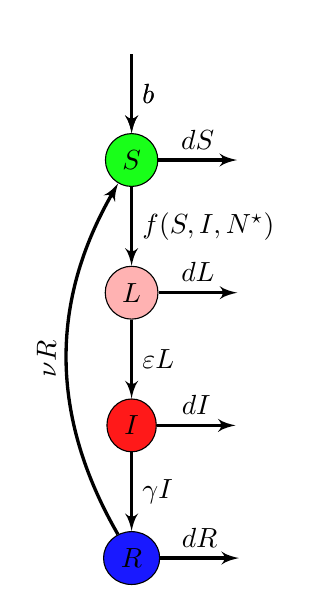
\begin{tikzpicture}[auto, %node distance = 2cm, auto,
	cloud/.style={minimum width={width("N-1")+2pt},
		draw, ellipse,fill=gray!20}]
    \node [cloud, fill=green!90] (S) {$S$};
    \node [cloud, below=of S, fill=red!30] (L) {$L$};
	\node [cloud, below=of L, fill=red!90] (I) {$I$};
	\node [cloud, below=of I, fill=blue!90] (R) {$R$};
    \node [cloud, above=of S, draw=none, fill=white] (b) {}; 
    \node [cloud, right=of S, draw=none, fill=white] (dS) {}; 
    \node [cloud, right=of L, draw=none, fill=white] (dL) {}; 
    \node [cloud, right=of I, draw=none, fill=white] (dI) {}; 
    \node [cloud, right=of R, draw=none, fill=white] (dR) {}; 
	%% Arrows
    \path [line, very thick] (b) to node [midway, right] (TextNode) {$b$} (S);
	\path [line, very thick] (S) to node [midway, right] (TextNode) {$f(S,I,N^\star)$} (L);
	\path [line, very thick] (L) to node [midway, right] (TextNode) {$\varepsilon L$} (I);
	\path [line, very thick] (I) to node [midway, right] (TextNode) {$\gamma I$} (R);
    \path [line, very thick, bend left] (R) to node [midway, above, sloped] (TextNode) {$\nu R$} (S);
	%% Birth and death
	\path [line, very thick] (b) to node [midway, right] (TextNode) {$b$} (S);
    \path [line, very thick] (S) to node [midway, above] (TextNode) {$dS$} (dS);
    \path [line, very thick] (L) to node [midway, above] (TextNode) {$dL$} (dL);
    \path [line, very thick] (I) to node [midway, above] (TextNode) {$dI$} (dI);
    \path [line, very thick] (R) to node [midway, above] (TextNode) {$dR$} (dR);
\end{tikzpicture}
\end{document}